%%%%%%%%%%%%%%%%%%%%%%%%%%%%%%%%%%%%%%%%%%%%%%%%%%%%%%%%%%%%%%%%%%%%%%%%%%%%%%%%
%%%%%%%%%%%%%%%%%%%%%%%%%%%%%%%%%%%%%%%%%%%%%%%%%%%%%%%%%%%%%%%%%%%%%%%%%%%%%%%%
%%                                                                            %%
%% opintnaytepohja.tex versio 3.01 (2017/10/06)                               %%
%% Opinnäytepohja käytettäväksi aaltothesis.sty (versio 3.01) -tyylitiedoston %%
%% kanssa.                                                                    %%
%% Toimiakseen paketti tarvitsee pdfx.sty v. 1.5.84 (2017/05/18) tai uudempi. %% 
%% The LaTeX template file to be used with the aaltothesis.sty (version 3.0)  %%
%% style file.                                                                %%
%% This package requires pdfx.sty v. 1.5.84 (2017/05/18) or newer.            %% 
%%                                                                            %%
%% This is licensed under the terms of the MIT license below.                 %%
%%                                                                            %%
%% Copyright 2017, by Luis R.J. Costa, luis.costa@aalto.fi,                   %%
%% Copyright 2017 documentation in Finnish in the template by Perttu Puska,   %%
%% perttu.puska@aalto.fi                                                      %%
%% Copyright Swedish translations 2014 by Elisabeth Nyberg,                   %%
%% elisabeth.nyberg@aalto.fi and Henrik Wallén, henrik.wallen@aalto.fi        %%
%%                                                                            %%
%% Permission is hereby granted, free of charge, to any person obtaining a    %%
%% copy of this software and associated documentation files (the "Software"), %%
%% to deal in the Software without restriction, including without limitation  %%
%% the rights to use, copy, modify, merge, publish, distribute, sublicense,   %%
%% and/or sell copies of the Software, and to permit persons to whom the      %%
%% Software is furnished to do so, subject to the following conditions:       %%
%% The above copyright notice and this permission notice shall be included in %%
%% all copies or substantial portions of the Software.                        %%
%% THE SOFTWARE IS PROVIDED "AS IS", WITHOUT WARRANTY OF ANY KIND, EXPRESS OR %%
%% IMPLIED, INCLUDING BUT NOT LIMITED TO THE WARRANTIES OF MERCHANTABILITY,   %%
%% FITNESS FOR A PARTICULAR PURPOSE AND NONINFRINGEMENT. IN NO EVENT SHALL    %%
%% THE AUTHORS OR COPYRIGHT HOLDERS BE LIABLE FOR ANY CLAIM, DAMAGES OR OTHER %%
%% LIABILITY, WHETHER IN AN ACTION OF CONTRACT, TORT OR OTHERWISE, ARISING    %%
%% FROM, OUT OF OR IN CONNECTION WITH THE SOFTWARE OR THE USE OR OTHER        %%
%% DEALINGS IN THE SOFTWARE.                                                  %%
%%                                                                            %%
%%                                                                            %%
%%%%%%%%%%%%%%%%%%%%%%%%%%%%%%%%%%%%%%%%%%%%%%%%%%%%%%%%%%%%%%%%%%%%%%%%%%%%%%%%

%% Käytä yksi näistä:
%% ensimmäinen, jos käytät pdflatexia, joka kääntää tekstin suoraan 
%% pdf-tiedostoksi (kuvat on oltava jpg-, png- tai pdf-tiedostoina. Kun teet
%% PDF/A-muotoista pdf-dokumenttia älä käytä PDF/A-muotoista tiedostoa kuvissa.)
%% ja haluat tulostaa opinnäytteesi
%% toinen, jos haluat verkkossa julkaistava PDF/A-muotoista tiedostoa
%% kolmas jos haluat tuottaa ps-tiedostoa (käytä eps-formaattia kuville, älä
%% käytä ps-muotoisia kuvia!)
%%
\documentclass[finnish, 12pt, a4paper, sci, utf8, pdfa]{aaltothesis}
%\documentclass[finnish, 12pt, a4paper, eng, utf8, pdfa, online]{aaltothesis}
%\documentclass[finnish, 12pt, a4paper, dvips]{aaltothesis}

\usepackage{graphicx}
\usepackage{amsfonts,amssymb,amsbsy}
\usepackage{amsmath}
\usepackage{enumitem}
\usepackage{array}
\usepackage{cellspace}
\usepackage{dsfont}
\usepackage[export]{adjustbox}

\newcolumntype{F}{>{\centering}p{0.15\textwidth}} % math-mode version of "l" column type

\newcommand{\Z}{\mathbb{Z}}
\newcommand{\N}{\mathbb{N}}
\newcommand{\indicator}{\mathopen{\mathds{1}}}
\newcommand*{\prob}{\mathbb{P}}

\newcommand{\subfigure}[2]{%
  \includegraphics[width=#2, valign=t, trim=2 2 2 2, clip]{#1}
}


%% Korjaa vastaamaan korkeakouluasi, jos automaattisesti asetettu nimi on 
%% virheellinen 
%%
%% Change the school field to specify your school if the automatically 
%% set name is wrong
% \university{aalto-yliopisto}
% \school{Sähkötekniikan korkeakoulu}

%% Korjaa seuraava vastaamaan koulutusohjelmaasi
%%
\degreeprogram{Teknillinen fysiikka ja matematiikka}
%%

%% Pääaineesi
\major{Matematiikka ja systeemitieteet}

%% Pääainekoodi
%%
\code{SCI3029}
%%

%% Valitse yksi näistä kolmesta
%%
\univdegree{BSc}
%%

%% Oma nimi
%%
\thesisauthor{Joonas Laukka}
%%

%% Opinnäytteen otsikko tulee tähän ja mahdollisesti uudelleen englannin- tai
%% ruostinkielisen abstraktin yhteydessä. Älä tavuta otsikkoa ja vältä liian
%% pitkää otsikkotekstiä. Jos latex ryhmittelee otsikon huonosti, voit joutua
%% pakottamaan rivinvaihdon \\ kontrollimerkillä.
%% Tällöin...
%% Muista että otsikkoja ei tavuteta! 
%% Jos otsikossa on ja-sana, se ei jää rivin viimeiseksi sanaksi vaan aloittaa
%% uuden rivin.
%% Anna ostikko uudelleen ilman rivinvaihtomerkkiä optionaalisena argumenttina
%% hakasuluissa. Näin tehdään, koska otsikko on osaa pdf/a-tiedostossa olevaa
%% metadataa, ja metadatassa ei saa olla rivinvaihtomerkkiä.
%%
\thesistitle{Satunnaiskävelyt ja niiden kasvattamat puut}
%\thesistitle[Opinnäytteen otsikko]{Opinnäyteen\\ otsikko}
%%

\place{Espoo}

%% Kandidaatintyön päivämäärä on sen esityspäivämäärä! 
%% 
\date{1.5.2018}
%%

%% Kandidaattiseminaarin vastuuopettaja tai diplomityön valvoja.
%% Huomaa tittelissä "\" -merkki pisteen jälkeen, ennen välilyöntiä ja
%% seuraavaa merkkijonoa. 
%% Näin tehdään, koska kyseessä ei ole lauseen loppu, jonka jälkeen tulee 
%% hieman pidempi väli vaan halutaan tavallinen väli.
%%
\supervisor{TkT\ Riikka Korte}
%%

%% Kandidaatintyön ohjaaja(t) tai diplomityön ohjaaja(t). Ohjaajia saa
%% olla korkeintaan kaksi.
%% 
%\advisor{Prof.\ Pirjo Professori}
\advisor{Prof.\ Lasse Leskelä}
%\advisor{DI Tina Tutkija}
%%

%% Aaltologo: syntaksi:
%% \uselogo{aaltoRed|aaltoBlue|aaltoYellow|aaltoGray|aaltoGrayScale}{?|!|''}
%% Logon kieli on sama kuin dokumentin kieli
%%
\uselogo{aaltoRed}{''}
%%

%% Suomenkielinen tiivistelmä:
%% Kaikki tiivistelmässä tarvittava tieto (nimesi, työnnimi, jne.) käytetään
%% niin kuin se on yllä määritelty.
%% Tiivistelmän avainsanat:
%% Huom! Avainsanat erotetaan toisistaan \spc -makrolla
%%
\keywords{Satunnaiskävely\spc puu\spc verkko\spc NRRW}

%% Tiivistelmän tekstiosa. Tämä teksti sisältyy pdf-tiedoston metadataa ja tulee
%% myös tiivistelmälomakkeeseen.
%%
\thesisabstract{
Nykymaailma on täynnä erilaisia verkkorakenteita Internetistä sosiaalisiin piireihin.
Verkkojen kasvun mallintaminen onkin kiinnittänyt tutkijoiden huomion kuluneen vuosikymmenen aikana.
Yksi tällainen kasvumalli on No Restart Random Walk (NRRW), jossa satunnaiskävelijä
kasvattaa suuntaamatonta verkkoa kulkiessaan siinä. Kävelijä lähtee alkusolmusta, kulkee s:n
kaaren läpi satunnaiseen solmuun, jonka naapuriksi lisätään uusi solmu. Uuden solmun asteluku on aina yksi. 
Tätä prosessia jatketaan satunnaiskävelijän viimeisimmästä tilasta, ja prosessin toistaminen kasvattaa satunnaisen puurakenteen. 
Mallin ominaisuudet määrää siis askelparametri, s. Tällainen NRRW-malli mukailee reaalimaailman verkoille tyypillisiä ominaisuuksia, 
kuten preferential and local attachment. Mallissa satunnaiskävelyprosessi
ja verkkoa kuvaavan satunnaisprosessi ovat voimakkaasti riippuvaisia. Prosessin käsittelyä
voidaan helpottaa osoittamalla, että se on yhdenmukainen yksinkertaisemman stokastisen prosessin kanssa.
Näytän, että NRRW-malli on stokastisesti yhdenmukainen rakentamani riippumattomien, tasajakautuneiden
satunnaislukujen määräämän mallin kanssa. Lopuksi käytän tätä vaihtoehtoista esitystapaa puun solmujen palautuvuutta
koskevan lauseen todistukseen.
}

%% Tekijänoikeusteksti. Tekijänoikeus on tekijällä riippumatta siitä onko
%% copyright -merkintä näkyvissä vai ei. Halutessasi voit jakaa työsi Creative 
%% Commons -lisensillä (katso creativecommons.org), jolloin lisenssitekstin on
%% oltava näkyvissä. Kirjoita tähän haluamasi tekijänoikeustekstin. Se kirjautuu
%% myös pdf-tiedoston metadataan.
%% Syntaksi:
%% \copyrigthtext{metadatateksti}{sivulle näkyviin tuleva teksti}
%% 
%% A.o. metadataan menevässä tekstissä on käytettävä \noexpand -makroa ennen
%% \copyright -erikoismerkkiä ja makrot (tässä \copyright ja \year) on erotettava 
%% seuraavasta tekstistä \ -merkillä (välilyöntimerkki). \copyrighttext-makron
%% argumentissa olevat makrot automaattisesti hakevat vuosiluvun ja tekijän nimi.
%% (Huom! \ThesisAuthor on aaltothesis.cls -tyylitiedoston sisäinen makro).
%% Toki saman tekstin olisi voinut kirjoittaa yksinkertaisesti näin:
%% \copyrighttext{Copyright \noexpand\copyright\ 2017 Teemu Teekkari}
%% {Copyright \copyright{} 2017 Teemu Teekkari}
%%
\copyrighttext{Copyright \noexpand\copyright\ \number\year\ \ThesisAuthor}
{Copyright \copyright{} \number\year{} \ThesisAuthor}

%% Voit estää LaTeXia kirjoittamasta xmpdata-tiedostoon (sisältää pdf-tiedostoon
%% kirjoitettavaa metadataa) asettamalla writexmpdatafile lipun arvoksi 'false'.
%% Tämä mahdollistaa sen, että voit kirjoittaa metadataa suoraan oikeassa
%% muodossa tiedostoon opinnaytepohja.xmpdata.
%%
%\setboolean{writexmpdatafile}{false}

%% Kaikki mikä paperille tulostuu, on tämän jälkeen
%%
\begin{document}
	
%% Tehdään kansilehti
%%
\makecoverpage

%% Tehdään tekijänoikeusteksti näkyväksi.
%% Halutessasi voit jättää tekijänoikeustekstin pois luettavasta pdf-tiedostosta. 
%% Tämä voi tuntua hyvältä ajatukselta paperille tulostetulla versiossa eteenkin,
%% jos sivun ainoa teksti on "Copyright (c) vvvv Teemu Teekkari". Suositus on
%% kuitenkin jättää teksti näkyviin.
%%
\makecopyrightpage

%% Suomenkielinen tiivistelmä
%% Kaikki tiivistelmässä tarvittava tieto (nimesi, työnnimi, jne.) käytetään
%% niin kuin se on yllä määritelty.
%%
%% Tiivistelmän tekstiosa
%%
\begin{abstractpage}[finnish]
Nykymaailma on täynnä erilaisia verkkorakenteita Internetistä sosiaalisiin piireihin.
Verkkojen kasvun mallintaminen onkin kiinnittänyt tutkijoiden huomion kuluneen vuosikymmenen aikana.
Yksi tällainen kasvumalli on \textit{No Restart Random Walk} (NRRW), jossa satunnaiskävelijä
kasvattaa suuntaamatonta verkkoa kulkiessaan siinä. Kävelijä lähtee alkusolmusta, kulkee \textit{s}:n
kaaren läpi satunnaiseen solmuun, jonka naapuriksi lisätään uusi solmu. Uuden solmun asteluku on aina yksi. 
Tätä prosessia jatketaan satunnaiskävelijän viimeisimmästä tilasta, ja prosessin toistaminen kasvattaa satunnaisen puurakenteen. 
Mallin ominaisuudet määrää siis askelparametri, \textit{s}.

Tällainen NRRW-malli mukailee reaalimaailman verkoille tyypillisiä ominaisuuksia, 
kuten \textit{preferential and local attachment}. Mallissa satunnaiskävelyprosessi
ja verkkoa kuvaavan satunnaisprosessi ovat voimakkaasti riippuvaisia. Prosessin käsittelyä
voidaan helpottaa osoittamalla, että se on yhdenmukainen yksinkertaisemman stokastisen prosessin kanssa.
Näytän, että NRRW-malli on stokastisesti yhdenmukainen rakentamani riippumattomien, tasajakautuneiden
satunnaislukujen määräämän mallin kanssa. Lopuksi käytän tätä vaihtoehtoista esitystapaa puun solmujen palautuvuutta
koskevan lauseen todistukseen.
\end{abstractpage}

%% \thesisabstract -makrossa kirjoitettu teksti on tallennettu \abstractext 
%% -makrosa jolloin voit siirtää metadataan menevä teksti sellaisenaan näin:
%%
%\begin{abstractpage}[finnish]
%	\abstracttext{}
%\end{abstractpage}

%% Pakotetaan uusi sivu varmuuden vuoksi, jotta mahdollinen suomenkielinen ja
%% englanninkielinen tiivistelmä eivät tule vahingossakaan samalle sivulle
%%
\newpage
%%
%% Opinnäytteen ostikko englanniksi. Poista, jos et tarvitse sitä.
\thesistitle{Random Walks and the Trees they Grow}
%\supervisor{Prof.\ Pirjo Professori}
\supervisor{DSc\ (Tech.) Riikka Korte}
\advisor{Prof.\ Lasse Leskelä}
\degreeprogram{Engineering Physics and Mathematics}
\department{Department of Mathematics and System Analysis}
\major{Mathematics and System Analysis}
%% Avainsanoja ei tarvitse erottaa \spc -makrolla.
\keywords{Random walk, graph, tree, NRRW}
%% Tiivistelmän tekstiosa
\begin{abstractpage}[english]
The modern world is full of networks from the Internet to social circles. Modeling the growth
of graphs has caught the attention of many researchers during the last decade. One such growth model
is a \textit{No Restart Random Walk} (NRRW). In an NRRW, a random walker grows
an undirected graph while it is traversing it. The walker starts from the root vertex and crosses \textit{s}
edges to end up in a random destination vertex. Then, a new vertex with degree 1 is added as its neighbour. 
This process is repeated starting from the destination vertex and consequently, a random tree is generated. 
The properties of the model are unambiguously determined by the step parameters, \textit{s}.

The NRRW model conforms to many properties that are common in real life graphs such as
preferential and local attachment. The random walk process and the random graph process are
mutually dependent. Examining these dependent processes can be simplified by proving that they
are equivalent with a simpler stochastic process. I will show that the NRRW model is stochastically
equivalent to a model seeded by a sequence of independent, uniformly distributed random numbers. Finally, I
will use this alternative model to prove a theorem about the recurrence of the vertices in an NRRW 
generated graph.
\end{abstractpage}

\newpage

\mysection{Esipuhe}


\vspace{5cm}
Otaniemi, 15.9.2017

\vspace{5mm}
{\hfill Joonas Laukka \hspace{1cm}}

%% Pakotetaan varmuuden vuoksi esipuheen jälkeinen osa
%% alkamaan uudelta sivulta
\newpage


%% Sisällysluettelo
%%
\thesistableofcontents


%% Symbolit ja lyhenteet
%%
\mysection{Symbolit ja lyhenteet}

\subsection*{Symbolit}

\begin{tabular}{ll}
$\N_{0}$  & ei-negatiiviset kokonaisluvut (\( 0, 1, 2, \ldots \))  \\
\end{tabular}

\subsection*{Operaattorit}

\begin{tabular}{ll}
   $ \indicator \left\{ X \right\} $               & indikaattorifunktio ehdolla X\\
   $ \prob \left[ X \right] $                      & tapahtuman X todennäköisyys\\
\end{tabular}

\subsection*{Lyhenteet}

\begin{tabular}{ll}
NRRW       & No Restart Random Walk\\
i.i.d.     & riippumaton ja identtisesti jakautunut\\
\end{tabular}


%% \clearpage on melkein samanlainen kuin newpage, mutta 
%% flushaa myös LaTeX:n floatit 
%% 
\cleardoublepage

%% Leipäteksti alkaa
%%
\section{Johdanto}

%% Ensimmäinen sivu tyhjäksi
%% 
\thispagestyle{empty}

TODO: Esimerkkejä reaalimaailman verkoista!

Mallin rakenne pyritään valitsemaan siten, että se mukailee parhaalla mahdollisella tavalla todellisia verkostoja. Niille on tyypillistä preferential ja local attachment sekä se, että verkon solmujen astejakauma ei ole eksponentiaalisesti rajoitettu (\textit{heavy-tailed distribution}). 
Yksi lupaava kasvumalli on \textit{No Restart Random Walk} (NRRW), jossa satunnaiskävelijä kasvattaa suuntaamatonta verkkoa kulkiessaan siinä. Nimen mukaisesti satunnaiskävely ei ala koskaan alusta, vaan jatkuu katkeamatta verkon kasvaessa. Prosessin ominaisuudet määrää askelparametri, s, ja se kehittyy seuraavanlaisen algoritmin mukaisesti:

\begin{enumerate}[noitemsep]
   \setcounter{enumi}{-1}
   \item Aluksi verkossa on yksi solmu, juuri, josta on kaari itseensä. Satunnaiskävelyn alkutila on juurisolmu.
   \item Satunnaiskävely ottaa s askelta verkossa.
   \item Verkkoon lisätään uusi solmu ja se liitetään satunnaiskävelyn senhetkiseen sijaintiin.
   \item Palataan kohtaan 1.
\end{enumerate}

Prosessin simulointi ja matemaattinen analyysi osoittaa, että parametrin s parillisuus vaikuttaa voimakkaasti satunnaiskävelyn ja satunnaisverkon luonteisiin:

\begin{table}[htb]
   \begin{center}
   \begin{tabular}{|c|c|p{7.5cm}|}
   \hline
   \textbf{Askelparametri} & \textbf{Satunnaiskävely} & \textbf{Satunnaisverkko} \\ \hline
   s = 1          & Väistyvä        & Solmujen asteluku on geometrisen jakauman stokastisesti dominoima. \\ \hline
   s = 2n         & Palautuva       & Sisäsolmujen asteluku ei ole eksponentiaalisesti rajoitettu. \\ \hline
   \end{tabular}
   \end{center}
\end{table}

NRRW-prosessi voidaan nähdä joko satunnaisena verkkona tai satunnaiskävelynä. Näkemyksestä riippumatta satunnaiskävelyn palautuvuus ja sen kasvattaman verkon luonne ovat kietoutuneet toisiinsa. Näiden toisistaan riippuvien prosessien käsittelyä voidaan helpottaa osoittamalla, että koko prosessi on yhdenmukainen yksinkertaisemman stokastisen prosessin kanssa. Tässä kandidaatin työssä näytän, että NRRW-prosessi on stokastisesti yhdenmukainen riippumattomien, tasajakautuneiden satunnaislukujen määräämän prosessin kanssa. Lopuksi käytän tätä vaihtoehtoista esitystapaa puun solmujen palautuvuutta koskevan lauseen todistukseen.

%% Opinnäytteessä jokainen osa alkaa uudelta sivulta, joten \clearpage
%%
\clearpage

\section{Malli}

\subsection{Yleiskatsaus}

NRRW-prosessi on kahden toisistaan riippuvan stokastisen prosessin pari, \( ( G_{t}^{s}, W_{t} )_{t \geq 0} \). Molemmat prosessit ovat kytkeytyneet vahvasti toisiinsa, mutta niitä voidaan jaksoittain tarkastella myös erillisinä. Taulukko \ref{realisaatio} esittää yhden mahdollisen NRRW-prosessin realisaation askelparametrilla \( s = 2 \) ja parillisilla ajanhetkillä.

\begin{table}[htb]
   \caption{Yksi mahdollinen NRRW-prosessin realisaatio askelparametrilla \( s = 2 \). Satunnaiskävely on harmaan värin osoittamassa tilassa ja uusi solmu on juuri lisätty sen naapuriksi. Satunnaiskävely siirtyi nykyiseen tilaansa alleviivatun solmun kautta. \label{realisaatio}}
   \begin{center}
   {\renewcommand{\arraystretch}{1.1}
   \begin{tabular}{|F|F|F|F|F|}
   \hline
   \subfigure{graphs/even_example/1.jpg}{14.8mm}
   &
   \subfigure{graphs/even_example/2.jpg}{14.8mm}
   & 
   \subfigure{graphs/even_example/3.jpg}{23.4mm}
   &
   \subfigure{graphs/even_example/4.jpg}{23.4mm}
   &
   \subfigure{graphs/even_example/5.jpg}{23.4mm}
   \tabularnewline
   \hline
   t = 0 & t = 2 & t = 4 & t = 6 & t = 8
   \tabularnewline
   \hline
   \end{tabular}
   }
   \end{center}
\end{table}

Askelparametri vaikuttaa huomattavasti siihen, millaisia verkkoja NRRW-prosessi kasvattaa. Tämä ilmenee hyvin tietokonesimuloiduista realisaatioista kuvassa \ref{simulaatiot}. Parametrilla \( s = 1 \) jokaiseen satunnäiskävelyn vierailemaan tilaan lisätään uusi solmu. Tämä johtaa korkeisiin puihin, joissa solmut jakutuvat tasaisesti parillisille ja parittomille tasoille. Satunnaiskävelyn kaikki tilat ovat väistyviä.

Sen sijaan parillinen askelparametri (\( s \in 2\N_{0} \)) johtaa hyvin toisenlaisiin verkkoihin. Simulaatiotulokset viittaavat solmujen kasaantuvan suurissa määrin joidenkin yksittäisten solmujen jälkeläisiksi. Kyseessä on niin sanottu \textit{prefential attachment} -ilmiö, jossa jotain mitattavaa suuretta kertyy sellaisille joukon alkioille, joilla on jo ennestään paljon kyseistä suuretta. Satunnaisverkossa tämä ilmenee siten, että uusia solmuja liitetään todennäköisimmin sellaisiin verkon solmuihin, joilla on jo ennestään korkea asteluku.

Parillisen askelparametrin NRRW-prosesseihin liittyy myös toinen erikoisuus. Koska uusi solmuja lisätään vain parillisen askelmäärän välein, niitä kertyy vain verkon parillisille tasoille, ellei satunnaiskävely kulje juurisolmun silmukkakaaren läpi. Silloin satunnaiskävelyn pariteetti vaihtuu ja uusia solmuja lisätään vain parittomille tasoille.

Parillisen askelparametrin NRRW-prosessin ominaisuudet vastaavat paremmin todellisia verkostoja, kuten Internettiä ja sosiaalisia piirejä [2]. Rajoitun siis tarkastelemaan vain parillisen askelparametrin NRRW-prosesseja.

\begin{figure}[htb]
\centering
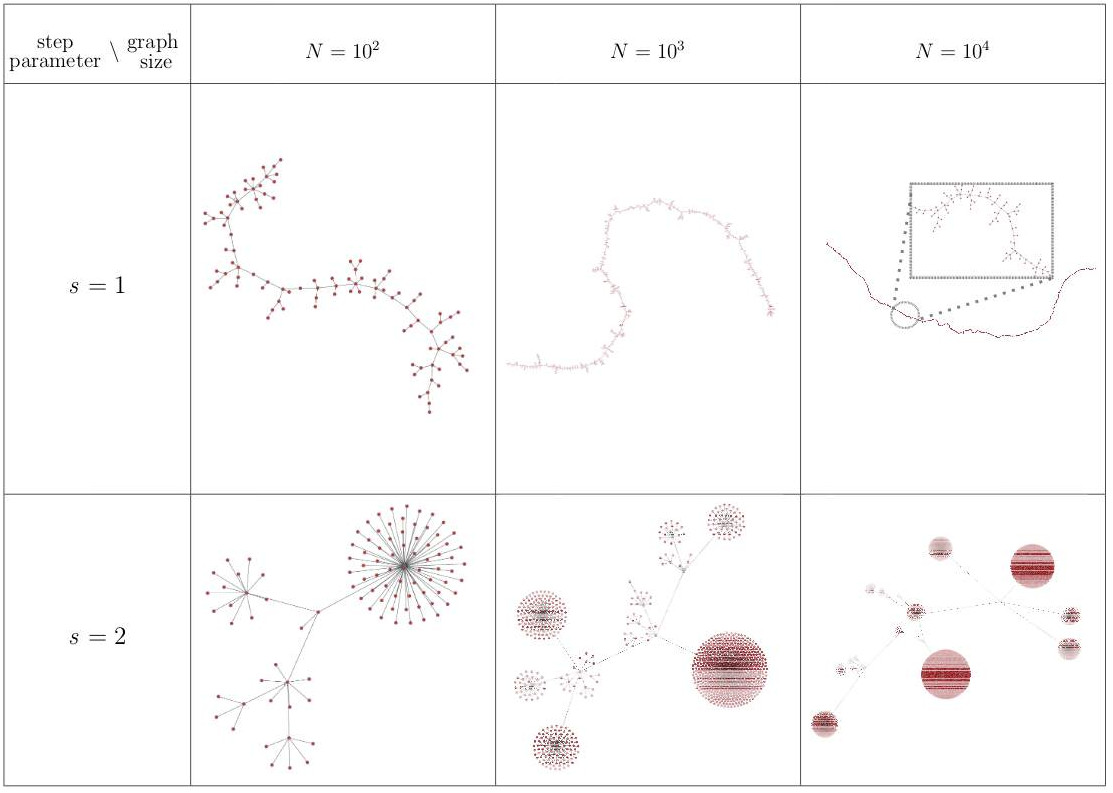
\includegraphics[width=.9\textwidth]{pictures/simulations.jpg}
\caption{NRRW-prosessin realisaatioita tietokonesimulaatioissa. [1] \label{simulaatiot}}
\end{figure}

\subsubsection{Satunnaisverkko}

\( G_{t}^{s} \), on satunnaisverkko, johon lisätään uusi solmu \textit{s} aikayksikön välein. Satunnaisprosessin tilajoukko on kaikkien suuntaamattomien, yhtenäisten ja syklittömien verkkojen eli puiden joukko.

\vspace{0.5cm}

\textbf{Määritelmä}: Suuntaamaton verkko G on pari (V, E), missä joukko V on verkon solmujen joukko (\( v_{i} \in V \)) ja E on suuntaamattomien kaarien joukko. Kaarien joukon alkiot ovat muotoa \( \{ v_{i}, v_{j} \} \). Kaari \( \{ v_{i}, v_{j} \} \) yhdistää solmut \( v_{i} \) ja \( v_{j} \) toisiinsa. 

\vspace{0.5cm}

Kasvavan verkon käsittelyn helpottamiseksi satunnaisverkon \( G_{t}^{s} \) solmut indeksoidaan kokonaisluvuilla (\( 0, 1, 2, \ldots \)) lisäysjärjestyksen mukaan. Juurisolmu on siis \( v_{0} \) ja hetkelä \( t = sn, \; n \in \Z \) lisätään solmu \( v_{n} \). Tarkastellaan satunnaisverkkoa \( (G_{t}^{s})_{t \geq 0} \) itsenäisenä prosessina. Sen siirtymätodennäköisyydet pois nykytilasta ovat nollasta poikkeavia vain ajanhetkillä \( t = sn, \; n \in \Z \). Ne määrää satunnaiskävelyn \( (W_{t})_{t \geq 0} \) siirtymämatriisi hetkellä \( t = sn \), \( P_{t} \):
\begin{equation}
\begin{split}
   & \prob \left[ G_{t+s}^{s} = (V_{t} \cup \{ v_{n + 1} \}, E_{t} \cup \{ (v_{i}, v_{n + 1}) \}) \mid G_{t} = (V_{t}, E_{t}) \right] \\
   &= \prob \left[ W_{t+s} = v_{i} \mid W_{t} = v_{n} \right] = (P_{t}^{s})_{n,i}
\end{split}
\end{equation}

\subsubsection{Satunnaiskävely}

Vastaavasti satunnaiskävelyprosessin \( (W_{t})_{t \geq 0} \) tilajoukon ja siirtymätodennäköisyydet määrää sen kasvattama satunnaisverkko. Molemmat näistä muuttuvat aina, kun verkkoon lisätään uusi solmu. Lisäyshetkien välillä tilajoukko on kuitenkin vakio ja satunnaiskävelyprosessi voidaankin silloin nähdä tavallisena äärellisen tilajoukon Markov-ketjuna. Jos satunnaiskävely on solmussa \( i \) hetkellä \( t \), valitaan seuraava tila satunnaisesti valitsemalla yksi solmusta \( i \) lähtevä kaari ja siirtymällä sen osoittamaan solmuun. Todennäköisyysmassa on tasajakautunut kaikkien solmun \( i \) kaarien kesken. 

Koska NRRW-prosessi rakentaa puita, ei verkossa ole muita syklejä, kuin juuren kaari itseensä. Verkkoteoriassa kaaret solmusta itseensä lasketaan kahdesti. Merkitään solmun \( v_{i} \) solmuun \( v_{j} \) yhdistävien kaarien määrää

\[
   \psi^{(t)}(v_{i}, v_{j}) = 
      \begin{cases}
         \indicator \left\{ \{ v_{i}, v_{j} \} \in E_{t} \right\} & \quad \text{jos } v_{i} \neq v_{j} \\
         2 \cdot \indicator \left\{ v_{i} = v_{0} \right\}        & \quad \text{muulloin}
      \end{cases}
   \label{equation:psi}
\]
missä \( E_{t} \) on verkon \( G_{t} \) kaarien joukko. Nyt todennäköisyys siirtyä solmusta \( v_{i} \) solmuun \( v_{j} \) on

\begin{equation}
   \prob \left[ W_{t+1} = v_{j} \mid W_{t} = v_{i} \right] = \frac{\psi^{(t)}(v_{i}, v_{j})}{d_{t}(v_{i})}
   \label{equation:verkko-tn}
\end{equation}
missä \( d_{t}(v_{i}) \) on solmun \( v_{i} \) asteluku hetkellä t. Toisin sanoen

\begin{equation}
   d_{t}(v_{i}) = \sum_{w \in V} \psi^{(t)}(v_{i}, w)
   \label{equation:asteluku}
\end{equation}
eli kaikkien solmuun \( v_{i} \) yhdistyvien kaarien lukumäärä.

\subsection{Kokonaisuus}

Satunnaisverkon ja satunnaiskävelyn erillinen tarkastelu paljastaa, että näistä jälkimmäinen on NRRW-prosessin keskeisin satunnaisuuden lähde. Satunnaiskävely muuttaa liikkeillään sen omaa tilajoukkoa eli verkkoa \( G_{t}^{s} \). Kun verkko muuttuu, myös satunnaiskävelyn siirtymätodennäköisyydet muuttuvat. Selvästi satunnaiskävelyprosessi on ajassa epähomogeeninen stokastinen prosessi. Satunnaisverkko sen sijaan kasvaa satunnaiskävelyn realisaation ohjaamana. Kokonaisuutena NRRW-prosessi on siis myös epähomogeeninen ajassa.

\subsection{Parillinen prosessi}

TODO: Erityishuomioita?

\section{Stokastinen esitys}

\subsection{Teoria}

Olkoon \( (\omega_{t})_{t \geq 0} \) jono riippumattomia välin \( [0, 1] \) tasajakautuneita satunnaislukuja. Toisin sanoen \( w_{t} \sim \text{Tas}(0, 1) \). Tällaista satunnaislukujen sarjaa voidaan käyttää monimutkaisemman stokastisen prosessin algoritmiseen simulointiin [3]. Simulointi rakennetaan etsimällä deterministinen funktio \( \phi : S \times [0, 1] \to S \), joka liittää stokastisen prosessin tilan ja välin \( [0, 1] \) reaaliluvun prosessin seuraavaan tilaan. Funktion \( \phi \) tulee toteuttaa yhtälö
\begin{align}
   \prob \left[ \phi(x, \omega_{t}) = y \right] &= \int\limits_0^1 \; \indicator \left\{ \phi(x, w) = y \right\} \mathrm{d}w \\
                                                &= \prob \left[ X_{t+1} = y \mid X_{t} = x \right] = P_{x,y} \quad \forall \; x, y \in S
   \label{equation:stokastinen-esitys}
\end{align}
Yhtälön \ref{equation:stokastinen-esitys} toteuttavaa funktiota \( \phi \) ja satunnaislukujonoa \( (\omega_{t})_{t \geq 0} \) kutsutaan siirtymämatriisin P \textit{stokastiseksi esitykseksi}.

Jos stokastisen prosessin alkutila on \( X_{0} = x_{0} \), sitä voidaan simuloida sen stokastisen esityksen avulla rekursiivisesti:
\begin{equation}
   X_{t+1} = \phi(X_{t}, \omega_{t})
\end{equation}

Mikäli stokastinen prosessi on epähomogeeninen ajassa, vaaditaan stokastiseen esitykseen jono deterministisiä funktioita \( (\phi^{(t)})_{t \geq 0} \), jotka ovat muotoa \( \phi^{(t)} : S \times [0, 1] \to S \; \forall \; t \geq 0 \). Funktioiden \( \phi^{(t)} \) tulee toteuttaa yhtälöä \ref{equation:stokastinen-esitys} vastaava ehto \( \forall \; t \geq 0 \):
\begin{equation}
   \prob \left[ \phi^{(t)}(x, \omega_{t}) = y \right] = \prob \left[ X_{t+1} = y \mid X_{t} = x \right] = P^{(t)}_{x,y} \quad \forall \; x, y \in S
   \label{equation:epahom-stokastinen-esitys}
\end{equation}

Prosessin simulointi tehdään, kuten homogeenisessa tilanteessa, mutta rekursiofunktio valitaan funktiojonosta \( (\phi^{(t)})_{t \geq 0} \) järjestyksessä:
\begin{equation}
   X_{t+1} = \phi^{(t)}(X_{t}, \omega_{t})
\end{equation}

\subsection{Propositio}

Edellä havaittiin, että NRRW-prosessi on epähomogeeninen ajassa. Sen stokastinen esitys on siis muotoa \( (\phi_{t}, \omega_{t})_{t \geq 0} \), missä funktiot \( \phi_{t} \) toteuttavat ehdon \ref{equation:epahom-stokastinen-esitys}. Muodostetaan sopiva jono deterministisiä funktioita NRRW-prosessille. Prosessin tilat ovat muotoa \( (v, G) \), missä \( G = (V, E) \) on verkko ja \( v \in V \) on verkon G solmu. Jakamalla rekursiofunktiot satunnaiskävely- ja satunnaisverkko-osiin saadaan niille korkeatasoinen muoto
\begin{equation}
   \phi^{(t)} \left( (v, G), w \right) = \left( \lambda^{(t)} \left( (v, G), w \right), \mu^{(t)} \left( \lambda^{(t)} \left( (v, G), w \right), G \right) \right)
\end{equation}
missä \( \lambda^{(t)} \) on satunnaiskävelyn \( (W_{t})_{t \geq 0} \) stokastisen esityksen rekursiofunktio ja \( \mu \) päivittää verkkoa G satunnaiskävelyn realisaation mukaisesti. Satunnaiskävelyn rekursiofunktio
\begin{equation}
   \lambda^{(t)} \left( (v, G), w \right) = 
   \begin{cases}
      v_{1} & w \in [0, \rho(G)_{i,1}) \\
      v_{2} & w \in [\rho(G)_{i,1}, \rho(G)_{i,1} + \rho(G)_{i,2}) \\
            & \quad \vdots \\
      v_{\lfloor \frac{t}{s} \rfloor} & w \in [\rho(G)_{i,\lfloor \frac{t}{s} \rfloor - 1}, \rho(G)_{i,\lfloor \frac{t}{s} \rfloor - 1} + \rho(G)_{i,\lfloor \frac{t}{s} \rfloor}) 
   \end{cases}
\end{equation}
missä \( \rho \) on funktio verkosta sen siirtymämatriisiin. Hyödyntäen määritelmän \ref{equation:psi} funktiota solmuja yhdistävien kaarien määrälle, saadaan kuvaukselle \( \rho \) alkioittainen määritelmä
\begin{equation}
   \rho^{(t)}(G)_{(i,j)} = \rho^{(t)} \left( (V, E) \right)_{(i,j)} = \frac{\psi^{(t)}(i, j)}{d_{t}(i)} = \frac{\psi^{(t)}(i, j)}{\sum_{w \in V} \psi^{(t)}(v_{i}, w)}
\end{equation}
missä kaksi viimeistä yhtäsuuruutta seuraa kaavoista \ref{equation:verkko-tn} ja \ref{equation:asteluku}.

Stokastisen esityksen verkkoa päivittävä funktio määritellään
\begin{equation}
   \mu^{(t)} \left( v, (V, E) \right) =
   \begin{cases}
      \left( V \cup {v_{t}}, E \cup \{ v, v_{t} \} \right) & \text{kun } t \bmod s = 0 \\
      \left( V, E \right) & \text{muulloin}
   \end{cases}
\end{equation}
Se siis lisää verkon solmuun \( v \) uuden solmun \( v_{t} \) aina kun aika on jaollinen askelparametrillä s. Muulloin verkkoa ei muuteta.

\subsection{Todistus}

Esitän, että stokastisen esityksen \( (\phi^{(t)}, \omega_{t})_{t \geq 0} \) simuloima stokastinen prosessi on todellakin NRRW-prosessi askelparametrillä s.


\subsection*{Rakenne}

Opinnäytteen rakenteen tulee olla hyvän tieteellisen kirjoittamisen käytännön
mukainen ja sisältää vähintään seuraavat osat:

\begin{enumerate}
\item Nimiölehti
\item Tiivistelmä
\item Sisällysluettelo
\item Symboli- ja lyhenneluettelo
\item \label{a} Johdanto
%% Tässä alla on esimerkki lainausmerkkien käytöstä. Suomalaisen tekstin
%% lainausmerkit eivät mene oikein latexissa (tai monissa muissakaan
%% julkaisujärjestelmissä) kun käytetään "-merkkiä, koska latex käyttää
%% amerikkalaista lainausmerkkien tulostustapaa. Vaihtoehtona voi käyttää
%% kulmalainausmerkkejä, jotka myös tulostuvat oikein.
\item  Aikaisempi tutkimus. Työn luonteen niin vaatiessa otsikko voi olla myös
        >>Teoreettinen tausta>>  tai näiden otsikoiden yhdistelmä.
\item Tutkimusaineisto ja -menetelmät %% yhdysmerkki - eli tavuviiva. 
\item Tulokset
\item \label{o} Tarkastelu. Työn luonteen niin vaatiessa otsikko voi olla myös
		>>Johtopäätökset>> tai >>Yhteenveto>> tai edellä mainittujen otsikoiden
		yhdistelmä.
\item Lähteet
\item Liitteet.
\end{enumerate}

Tiivistelmän ja symboli- sekä lyhenneluetteloiden väliin voi sijoittaa
halutessaan esipuheen.  

Työn osat \ref{a}--\ref{o} muodostavat \textit{tekstiosan.}  Työn yksittäisiä
osia voidaan jakaa alaotsikoilla alaosiin, joita ei ole yllä esitetty. 
Alaotsikoiden käyttäminen selventää parhaimmillaan tekstiä, ja pahimmillaan 
sirpaloittaa sitä.  Sirpaloitumista voi estää huolehtimalla siitä, että samalla 
sivulla ei esiinny useampaa alaotsikkoa. Tekstin jäsentelyssä on yleensä 
ongelmia, jos osassa on vain yksi alaosa, tai kirjoittaja joutuu käyttämään 
useampaa kuin kahta tasoa (osa ja alaosat): alaosien alaosat ovat harvoin tarpeen.

\subsection*{Sivut ja kirjaintyypit}

Opinnäytteen tulee olla kirjoitettu koneella tai
tekstinkäsittelyohjelmalla yksipuolisesti A4-kokoiselle paperille.
Kandidaatintyön tekstiosan sopiva pituus on noin 15--20 sivua ja
diplomityön noin 60 sivua. Työtä ei ole syytä tarpeettomasti pidentää.

Opinnäytteen tekstiosan kirjaintyypin tulee olla antiikva eli
%% esimerkki pakkotavutuksesta; "serif-tyyppinen" on tavutuksen kannalta
%% hankala, joten pakkotavutetaan se. 
serif\--tyyp\-pi\-nen ja lisäksi kursivoimaton, lihavoimaton sekä kooltaan 12
pistettä (kuten tässä esityksessä). Groteskeja eli \textsf{Sans serif}-tyyppisiä
kirjaintyyppejä (kuten Helvetica tai Arial) ei saa käyttää varsinaisessa
tekstissä, mutta otsikoissa näitä voidaan käyttää.  Otsikoissa voidaan käyttää
kooltaan edellä mainittua suurempaa kirjaintyyppiä sekä tyylikeinoja, kuten
lihavointia tai kursivointia. Tekstissä samantasoisten otsikoiden on kuitenkin
oltava tyyliltään ja kirjainlajeiltaan yhteneväisiä.

%% Esimerkki taulukosta
\begin{table}[htb]
%% Taulukon teksti
\caption{Taulukoissa ja kuvissa kirjaintyypin voi valita
tarkoituksenmukaisesti, mutta kuva- ja taulukkoteksteissä tulee
käyttää samaa kirjaintyyppiä kuin varsinaisessa tekstissä. 
Huomaa taulukon numeroinnin sijoittuminen taulukon yläpuolelle. \label{taulukko1}}
\begin{center}
\fbox{
\begin{tabular}{c|l|r}
\textbf{A} & 1 & $e^{j \omega t}$ \\ \hline
\textsf{B} & 2 & ${\mathfrak R}(c)$ \\ \hline
\texttt{C} & 3 & $ a \in \mathbb{A}$  
\end{tabular}
}
\end{center}
\end{table}

Opinnäytteen vasen marginaali (sidonnan puoli) on
35~mm % tässä ~ muodostaa ns. yhdistävän välilyönnin
ja oikea 25~mm. Ylämarginaali on 25~mm. Leipätekstin korkeus on
enimmillään 230mm. Tämän opinnäytepohjan marginaalien pitäisi olla
paperille tulostettuna oikein, mutta tulostimesta ja paperista
riippuen voi esiintyä yhden tai kahden millimetrin suuruisia eroja.
%% Jos käännät tämän tekstin pdflatex-komennolla ja tulostat sen katselu-
%% ohjelmasta, toteat todennäköisesti em. mittojen poikkeavan enemmän
%% kuin 1-2 mm. 
%% Tämä on seurausta pdf-tiedoston erilaisesta kirjaintyyppimäärityksestä.
%% Korkeatasoista painotyötä varten käytä vain latex-komentoa ja 
%% tulosta postscript-muotoon käännetystä tiedostosta. 
\subsection*{Asemointi}

%% Muutos vanhaan ohjeeseen verrattuna: aikaisemmassa ohjeessa
%% kehotettiin käyttämään vasensuora-asettelua, mutta tässä
%% ohjeessa ollaan luovuttu tuosta vaatimuksesta ja siirrytty
%% huoliteltumpaan, painotuotteenomaisempaan suuntaan.  
Tekstiosan tekstissä käytetään kappaleiden erottamiseen sisennystä,
mutta ensimmäistä otsikon, väliotsikon tai muun katkon jälkeistä
kappaletta ei sisennetä. Jos kuva tai muu katko tulee kappaleiden
väliin, suositellaan katkon jälkeisen kappaleen sisentämistä.

Mikäli oikea reuna halutaan tasata, tulee käyttää tavutusta ja lisäksi
tarkistaa, ettei tekstiin jää lukemista häiritseviä pitkiä sanavälejä. Jos
käytät opinnäytteen tekemisessä \LaTeX-järjestelmää, 
tämä asia hoituu automaattisest.

Opinnäytteen riviväli on 1, mikä on myös tämän opinnäytepohjan käytäntö. 
Kappaleiden tulee yleensä olla ainakin kolmen rivin pituisia, mutta
myös liian pitkiä kappaleita tulee välttää.  Tässä opinnäytepohjassa
ei tekstin luonteen vuoksi voida täysin toteuttaa kappaleen pituutta koskevia
vaatimuksia.

Yksittäisiä, kappaleen päättäviä tai aloittavia rivejä sivun alussa
tai lopussa on vältettävä koko työssä, myös luetteloissa ja
liitteissä.

\subsection*{Numerointi}

Opinnäytteen jokainen osa alkaa uudelta sivulta. Alaosa aloittaa uuden
sivun vain edellisen sivun täytyttyä.

Työn osat numeroidaan siten, että johdanto on ensimmäinen numeroitava
osa. Osien numeroinnissa käytetään arabialaisia numeroita.

Nimiölehti, tiivistelmä, esipuhe, sisällysluettelo ja symboli- ja
lyhenneluettelo numeroidaan esipuheesta tai tämän puuttuessa 
ensimmäiseltä luettelosivulta alkaen roomalaisin numeroin.

Sivunumerointi alkaa toiselta varsinaiselta tekstisivulta, ja 
sivunumeroinnissa käytetään arabialaisia numeroita.

Lähdeluettelo alkaa uudelta sivulta. Lähdeluettelon sivunumerointi 
jatkuu viimeisestä tekstisivusta.

Jokainen liite alkaa uudelta sivulta. Liitteiden sivunumerointi
jatkuu viimeisestä lähdeluettelon sivusta.

Sivunumero sijoitetaan sivun yläreunaan.

Matemaattiset kaavat numeroidaan arabialaisin
numeroin. Kaavanumerointi ei saa katketa osien välissä (eikä niin
tapahdukaan, jos käytät tätä opinnäytepohjaa). Kaikkia kaavoja ei tarvitse
numeroida, vaan kirjoittaja voi käyttää harkintaa numeroinnin
tarpeellisuudessa.  Liitteissä olevat kaavat numeroidaan siten, että
liitteen ajatellaan muodostavan numeroinnin kannalta itsenäisen ja
yhtenäisen kokonaisuuden. Kaavan numero sijoitetaan oikealle puolelle
alla olevan esimerkin mukaisesti
\begin{equation}
D(xy) = (Dx)y + x(Dy),  \hspace{3em} x,y \in \mathbb{A}.
\end{equation}
%% Kaavojen jälkeen ei yleensä laiteta sisennystä. 
Kaikki kuvat ja taulukot numeroidaan erillisen juoksevan numeroinnin
mukaisesti kuten taulukosta \ref{taulukko1} ja kuvasta \ref{kuva1} käy
ilmi.  Liitteissä olevat kuvat ja taulukot numeroidaan siten, että
liitteen ajatellaan muodostavan numeroinnin kannalta itsenäisen ja
yhtenäisen kokonaisuuden. Liitteissä \ref{LiiteA} ja \ref{LiiteB} on
esimerkkejä kaavojen (kaavat \ref{liitekaava1}--\ref{liitekaava2} tai
kaavat \ref{liitekaava3}--\ref{liitekaava4}), kuvien (kuva
\ref{liitekuva}) ja taulukoiden (taulukko \ref{liitetaulukko})
numeroimisesta.  Liitteet numeroidaan suuraakkosin (esimerkiksi Liite
A, Liite B tai pelkästään A, B).
%% Tässä esimerkki kuva1.pdf -nimisen tiedoston tuomisesta kuvaksi.
%% Komento \inclugraphics[parametrit]{argumentti} tuo kuvan.
%% Komento \centering pakottaa kuvan keskelle. 
%% Komento \caption luo kuvatekstin ja sen numeroinnin
%% Parametrit htb pakottavat kuvan suunnilleen siihen 
%% kohtaan, missä se esiintyy tekstin lähdekoodissa
\begin{figure}[htb]
\centering
%\includegraphics[height=5cm]{./kuva1pdfa}
%\includegraphics[height=5cm]{./kuva1.pdf}
%\includegraphics[height=5cm]{./kuva1.jpg}
%\includegraphics[height=5cm]{./kuva1.png}
\caption{Tämä on esimerkki numeroidusta kuvatekstistä. \label{kuva1}}
\end{figure}

\subsection*{Lähdeviittausten käyttö} 

Lähdeviittaukset tulee tehdä huolellisesti ja johdonmukaisesti
numeroviitejärjestelmän mukaisesti. Numeroviitteet järjestetään
lähdeluetteloon viittausjärjestykseen, mutta jos lähdeluettelo
on hyvin laaja (useita sivuja), järjestetään viitteet pääsanan 
mukaiseen aakkosjärjestykseen. Alaviitejärjestelmää
\footnote{Myöskään alaviitteenä olevia kommentteja \underline{ei} suositella
käytettäviksi.} ei käytetä. 

Viitteen sijoittelussa noudatetaan seuraavia sääntöjä:
Jos viite kohdistuu vain yhteen virkkeeseen tai virkkeen 
osaan, viite \cite{Kauranen} sijoitetaan virkkeen sisään ennen virkettä
päättävää pistettä. Jos taas viite koskee tekstin useampaa
virkettä tai kokonaista kappaletta, sijoitetaan viite kappaleen loppuun 
pisteen jälkeen. \cite{Kauranen} 

\subsection*{Lähdeluettelo} 

Lähdeluettelossa esiintyy tavallisesti seuraavassa esitettäviä
lähteitä, joista on numeroviitejärjestelmässä ilmoitettava
asianomaisessa kohdassa vaaditut tiedot.

%% Esimerkki korostamisesta. Lihavoinnin sijasta on tyylikkäämpää
%% ja luettavampaa käyttää kursiivia.
\textit{Kirjasta} ilmoitetaan seuraavat tiedot:

\begin{itemize}
\item[--]tekijät 
\item[--]julkaisun nimi
\item[--]painos, jos useita
\item[--]kustannuspaikka
\item[--]julkaisija tai kustantaja
\item[--]julkaisuaika
\item[--]mahdollinen sarjamerkintö. 
\end{itemize}

Viitteet \cite{Kauranen}--\cite{Koblitz} ovat esimerkkejä kirjan
esittämisestä lähdeluettelossa. Viite \cite[s.\ 83--124]{Koblitz} on
esimerkki lähdeluettelossa esiintyvän kirjan tiettyjen sivujen
esittämisestä tekstissä.

\textit{Artikkelista} kausijulkaisussa ilmoitetaan seuraavat tiedot:

\begin{itemize}

\item[--]tekijät
\item[--]artikkelin nimi
\item[--]kausijulkaisun nimi
\item[--]julkaisuvuosi
\item[--]kausijulkaisun volyymi tai ilmestymisvuosi
\item[--]kausijulkaisun numero
\item[--]sivut, joilla artikkeli on.
\end{itemize}

Viitteet \cite{bcs}--\cite{Deschamps} ovat esimerkkejä artikkelin
esittämisestä lähdeluettelossa.

\textit{Kokoomateoksen luvusta tai osasta} ilmoitetaan seuraavat tiedot:

\begin{itemize}
\item[--]luvun tai osan tekijät
\item[--]luvun tai osan nimi
\item[--]maininta >>Teoksessa>>
\item[--]koko teoksen toimittajat sekä maininta >>(toim.)>>
\item[--]koko teoksen tai konferenssin nimi
\item[--]konferenssiesitelmän kyseessä ollessa sen pitopaikka ja -aika
\item[--]painos, jos useita
\item[--]kustannuspaikka
\item[--]julkaisija tai kustantaja, jos aihetta tämän ilmoittamiseen on
\item[--]julkaisuaika
\item[--]sivut, joilla luku tai osa on 
\item[--]mahdollinen sarjamerkintä.
\end{itemize}

Viitteet \cite{Sihvola}--\cite{Lindblom} ovat esimerkkejä
kokoomateoksen luvun tai osan esittämisestä lähdeluettelossa. 

\textit{Opinnäytetyöstä} ilmoitetaan seuraavat tiedot:

\begin{itemize}
\item[--]tekijä
\item[--]työn nimi
\item[--]opinnäytetyön tyyppi
\item[--]oppilaitoksen nimi
\item[--]osaston, laitoksen tai ohjelman nimi
\item[--]oppilaitoksen sijaintipaikka
\item[--]vuosiluku.
\end{itemize}

Viitteet \cite{Miinusmaa}--\cite{Lonnqvist} ovat esimerkkejä
opinnäytteen esittämisestä lähdeluettelossa. 

\textit{Standardista} ilmoitetaan seuraavat tiedot:

\begin{itemize}
\item[--]standardin tunnus ja numero
\item[--]standardin nimi
\item[--]painos, mikäli ei ole ensimmäinen
\item[--]julkaisupaikka
\item[--]julkaisija
\item[--]julkaisuvuosi
\item[--]sivumäärä.
\end{itemize}
Viite \cite{sfs} on esimerkki standardin esittämisestä opinnäytteen
lähdeluettelossa. 

\textit{Haastattelusta} ilmoitetaan seuraavat tiedot:

\begin{itemize}
\item[--]haastatellun henkilön nimi
\item[--]haastatellun henkilön arvo tai asema
\item[--]haastatellun henkilön edustama organisaatio
\item[--]organisaation osoite
\item[--]maininta siitä, että kyseessä on haastattelu ja haastattelun
päivämäärä. 
\end{itemize}

Viite \cite{haastattelu} on esimerkki 
haastattelun esittämisestä lähdeluettelossa.

Osa sähköisessä muodossa olevista artikkeleista on saatavissa myös
painettuina. \textit{Vain verkosta saatavissa olevasta artikkelista} esitetään
seuraavat tiedot:

\begin{itemize}
\item[--]tekijät
\item[--]artikkelin nimi
\item[--]kausijulkaisun nimi
\item[--]viestintyyppi
\item[--]laitos tai volyymi
\item[--]kausijulkaisun yksittäistä osaa koskeva merkintä tai numero
\item[--]julkaisuvuosi tai maininta >>Päivitetty>> ja päivitysaika
\item[--]maininta >>Viitattu>> ja viittaamisen ajankohta 
\item[--]maininta >>Saatavissa>> ja URL tai 
        maininta >>DOI>> ja DOI-numero (DOI=Digital Object Identifier).
\end{itemize}

Viitteet \cite{Ribeiro}--\cite{kone} ovat esimerkkejä sähköisessä
muodossa olevan artikkelin esittämisestä opinnäytteen
lähdeluettelossa.  Viitteet \cite{Ribeiro} ja \cite{Stieber} ovat
saatavissa sekä painettuna että verkosta, joten viitteiden esitystapa
mukailee painetun artikkelin viitteen esitystapaa, mutta sen lisäksi
kerrotaan julkaisun olevan verkkolehti ja lehden olevan saatavissa
myös painettuna.  Viite \cite{kone} on saatavissa vain verkosta ja
siitä esitetään yllä vaaditut tiedot.

Valitettavasti sähköisessä muodosssa olevasta artikkelista ei ole aina 
saatavissa lai\-tos-, volyymi- tai numerotietoja.

\textit{Sähköisessä muodossa olevasta opinnäytetyöstä} ilmoitetaan
seuraavat tiedot:
 
\begin{itemize}
\item[--]tekijä
\item[--]työn nimi
\item[--]viestintyyppi
\item[--]opinnäytetyön tyyppi
\item[--]oppilaitoksen nimi
\item[--]osaston, laitoksen tai ohjelman nimi
\item[--]oppilaitoksen sijaintipaikka
\item[--]vuosiluku
\item[--]viittamisen ajankohta
\item[--]maininta "Saatavissa" ja URL tai 
        maininta "DOI" ja DOI-numero.
\end{itemize}

Viite \cite{Adida} on esimerkki sähköisessä muodossa olevan
opinnäytteen esittämisestä lähdeluettelossa.

Viite \cite{viittaaminen} on esimerkki itsenäisen kirjoituksen sisältävästä
verkkosivusta. Tällainen lähde on rinnastettavissa erillisteokseen.
\textit{Verkkosivusta} esitetään tiedot:

\begin{itemize}
\item[--] tekijät
\item[--] otsikko
\item[--] maininta "Päivitetty" ja päivitysaika 
\item[--] maininta "Viitattu" ja viittaamisen ajankohta
\item[--] Maininta "Saatavissa" ja URL.
\end{itemize}

Joskus verkkosivun kirjoitus on jaettu useammalle sivulle, jolloin
lähdeluetteloon kirjataan vain sellainen verkko-osoite, joka koskee
koko kirjoitusta tai sen etusivua, ellei sitten 
todella tarkoiteta kirjoituksen yksittäistä sivua. 

\subsection*{Muuta huomioitavaa lähdeluettelossa}

%% Muutos vanhoihin ohjeisiin koskien kieltä.
Lähdeluettelossa työn ja julkaisun nimi kirjoitetaan alkuperäisessä
muodossaan. Julkaisijan kotipaikka kirjoitetaan alkukielisessä
muodossaan.

Viittamista koskevassa suomalaisessa standardissa
SFS 5342 \cite{sfs} vaaditaan julkaisuista ilmoitettavaksi myös ISBN- tai
ISSN-numerot, mutta näissä opinnäyteohjeissa ei ISBN- ja 
ISSN-numeroita vaadita. 

\clearpage

\section{Tutkimusaineisto ja -menetelmät}

Tässä osassa kuvataan käytetty tutkimusaineisto ja tutkimuksen metodologiset
valinnat, sekä kerrotaan tutkimuksen toteutustapa ja käytetyt menetelmät.

\clearpage

\section{Tulokset}

Tässä osassa esitetään tulokset ja vastataan tutkielman alussa
esitettyihin tutkimuskysymyksiin. Tieteellisen kirjoitelman
arvo mitataan tässä osassa esitettyjen tulosten perusteella. 

%% Huomaa seuraavassa kappaleessa lainausmerkkien ulkopuolella piste, 
%% koska piste ei lopeta lainattua tekstinpätkää.
%% Jos lainattu tekstinpätkä loppuu välimerkkiin, tulee välimerkki
%% lainausmerkkien sisälle: 
%% "Et tu, Brute?" sanoi Caesar kuollessaan.
Tutkimustuloksien merkitystä on aina syytä arvioida ja tarkastella
kriittisesti.  Joskus tarkastelu voi olla tässä osassa, mutta se
voidaan myös jättää viimeiseen osaan, jolloin viimeisen osan nimeksi
tulee >>Tarkastelu>>. Tutkimustulosten merkitystä voi arvioida myös
>>Johtopäätökset>>-otsikon alla viimeisessä osassa. 

Tässä osassa on syytä myös arvioida tutkimustulosten luotettavuutta.
Jos tutkimustulosten merkitystä arvioidaan >>Tarkastelu>>-osassa,
voi luotettavuuden arviointi olla myös siellä. 

\clearpage

\section{Yhteenveto}
%\section{Summary} 

Opinnäytteen tekijä vastaa siitä, että opinnäyte on tässä dokumentissa
ja opinnäytteen tekemistä käsittelevillä luennoilla sekä
harjoituksissa annettujen ohjeiden mukainen muotoseikoiltaan,
rakenteeltaan ja ulkoasultaan.



\clearpage
%% Lähdeluettelo

\thesisbibliography

\begin{thebibliography}{99}

%% Alla pilkun jälkeen on pakotettu oikea väli \<välilyönti>-merkeillä.
\bibitem{Kauranen} Kauranen,\ I., Mustakallio,\ M. ja Palmgren,\ V.
  \textit{Tutkimusraportin kirjoittamisen opas opinnäytetyön
    tekijöille.}  Espoo, Teknillinen korkeakoulu, 2006.

\bibitem{Itkonen} Itkonen,\ M. \textit{Typografian käsikirja.} 3.\
  painos.  Helsinki, RPS-yhtiöt, 2007.

\bibitem{Koblitz} Koblitz,\ N. \textit{A Course in Number Theory and
    Cryptography. Graduate Texts in Mathematics 114.}  2.\ painos. New
  York, Springer, 1994.

%% Kun on useampi nimikirjain, jokaisen nimikirjaimen väliin
%% kuuluu välilyönti. Oikea välin määrä on saatu \<välilyönnillä>
\bibitem{bcs} Bardeen,\ J., Cooper,\ L.\ N. ja Schrieffer,\ J.\ R.
  Theory of Superconductivity. \textit{Physical Review,} 1957, vol.\
  108, nro~5, s.\ 1175--1204.

\bibitem{Deschamps} Deschamps,\ G.\ A. Electromagnetics and
  Differential Forms. \textit{Proceedings of the IEEE,} 1981, vol.\
  69, nro~6, s.\ 676--696.

%% Alla esimerkki englanninkielisen tavuttamisen pakottamisesta.
%% Oletusarvoisesti käytetään suomalaista tavutusta, mutta viitteissä
%% esiintyy usein muunkielisiä lauseita, jotka tulevat siten tavutetuksi
%% suomen kielen sääntöjen mukaan. Tämän voi korjata \foreignlanguage-
%% komennolla, jonka ensimmäinen parametri on vieraan kielen nimi ja toinen 
%% on vieraalla kielellä tavutettava teksti. 
\bibitem{Sihvola} Sihvola,\ A.\ et al.
  \foreignlanguage{english}{Interpretation of measurements of helix 
    and bihelix superchiral structures.}
  Teoksessa: Jacob,\ A.\ F. ja
  Reinert,\ J. (toim.) \textit{Bianisotropics '98 7th International
    Conference on Complex Media.}  Braunschweig, 3.--6.6.1998.
  Braunscweig, Technische Universität Braunschweig, 1998, s.\
  317--320.

%% Alla on suomalainen yhdistelmäsukunimi. Sen nimien välissä 
%% käytetään yhdysmerkkiä l. tavuviivaa, kirjoitetaan -.
\bibitem{Lindblom} Lindblom-Ylänne,\ S. ja Wager,\ M.  Tieteellisten
  opinnäytetöiden ohjaaminen. Teoksessa: Lindblom-Ylänne,\ S. ja
  Nevgi,\ A. (toim.) \textit{Yliopisto- ja korkeakouluopettajan
    käsikirja.}  Helsinki, WSOY, 2004, s.\ 314--325.
 
\bibitem{Miinusmaa} Miinusmaa,\ H. Neliskulmaisen reiän poraamisesta
  kolmikulmaisella poralla. Diplomityö, Teknillinen korkeakoulu,
  konetekniikan osasto, Espoo, 1977.

%% Tässä taas pakotettu englanninkielinen tavutus. 
%% Pedanttinen kirjoittaja pakottaa tietysti jokaiseen englanninkieliseen
%% lauseeseen englannin tavutuksen, mutta tässä esityksessä ei näin ole
%% tehty selvyyden ja lähdekoodin luettavuuden takia. 
\bibitem{Loh} Loh,\ N.\ C. High-Resolution Micromachined
  Interferometric Accelerometer. Master's Thesis, Massachusetts
  Institute of Technology, Cambridge,
  \foreignlanguage{english}{Massachusetts,} 1992.

\bibitem{Lonnqvist} Lönnqvist,\ A.
  \foreignlanguage{english}{Applications of hologram-based compact
    range: antenna radiation pattern, radar cross section, and
    absorber reflectivity measurements.}
  Väitöskirja, Teknillinen korkeakoulu, sähkö- ja tietoliikennetekniikan
  osasto, 2006.

\bibitem{sfs} SFS 5342. Kirjallisuusviitteiden laatiminen. 2.\ painos.
  Helsinki, Suomen standardisoimisliitto, 2004. 20~s.

\bibitem{haastattelu} Palmgren,\ V. Suunnittelija. Teknillinen
  korkeakoulu, kirjasto. Otaniementie 9, 02150 Espoo. Haastattelu
  15.1.2007.

\bibitem{Ribeiro} Ribeiro,\ C.\ B., Ollila,\ E. ja Koivunen,\ V.
  \foreignlanguage{english}{Stochastic Maximum-Likelihood Method for
    MIMO Propagation Parameter Estimation.}
 \textit{IEEE Transactions
    on Signal Processing,} verkkolehti, vol.\ 55, nro~1, s.\ 46--55.
  Viitattu 19.1.2007. Lehti ilmestyy myös painettuna. DOI:
  10.1109/TSP.2006.882057.

\bibitem{Stieber} Stieber,\ T. GnuPG Hacks. \textit{Linux Journal,}
  verkkolehti, 2006, maaliskuu, nro~143. Viitattu 19.1.2007. Lehti
  ilmestyy myös painettuna. Saatavissa:
  \url{http://www.linuxjournal.com/article/8732.}

\bibitem{kone} Pohjois-Koivisto,\ T. Voiko kone tulevaisuudessa arvata
  tahtosi?  \textit{Apropos,} verkkolehti, helmikuu, nro~1, 2005.
  Viitattu 19.1.2007.  Saatavissa:
  \url{http://www.apropos.fi/1-2005/prima.php.}

\bibitem{Adida} Adida,\ B.  Advances in Cryptographic Voting Systems.
  Verkkodokumentti. Ph.D.\ Thesis, Massachusetts Institute of
  Technology, Cambridge, 
  \foreignlanguage{english}{Massachusetts,}
  2006. Viitattu 19.1.2007.  Saatavissa:
  \url{http://crypto.csail.mit.edu/~cis/theses/adida-phd.pdf.}

\bibitem{viittaaminen} Kilpeläinen,\ P. WWW-lähteisiin viittaaminen
  tutkielmatekstissä. Verkkodokumentti. Päivitetty 26.11.2001.
  Viitattu 19.1.2007. Saatavissa:
  \url{http://www.cs.uku.fi/~kilpelai/wwwlahteet.html.}

\end{thebibliography}

%% Liitteet
%% Jos liitteitä ei ole, poista a.o. \clearpage- ja \thesisappendix -makrot.
\clearpage

\thesisappendix

\section{Esimerkki liitteestä\label{LiiteA}}

Liitteet eivät ole opinnäytteen kannalta välttämättömiä ja 
opinnäytteen tekijän on 
kirjoittamaan ryhtyessään hyvä ajatella pärjäävänsä ilman liitteitä.
Kokemattomat kirjoittajat, jotka ovat huolissaan
tekstiosan pituudesta, paisuttavat turhan 
helposti liitteitä pitääkseen tekstiosan pituuden annetuissa rajoissa.
Tällä tavalla ei synny hyvää opinnäytettä.   

Liite on itsenäinen kokonaisuus, vaikka se täydentääkin tekstiosaa.
Liite ei siten ole pelkkä listaus, kuva tai taulukko, vaan 
liitteessä selitetään aina sisällön laatu ja tarkoitus. 

Liitteeseen voi laittaa esimerkiksi listauksia. Alla on 
listausesimerkki tämän liitteen luomisesta. 

%% Verbatim-ympäristö ei muotoile tai tavuta tekstiä. Fontti on monospace.
%% Verbatim-ympäristön sisällä annettuja komentoja ei LaTeX käsittele. 
%% Vasta \end{verbatim}-komennon jälkeen jatketaan käsittelyä.
\begin{verbatim}
	\clearpage
	\appendix
	\addcontentsline{toc}{section}{Liite A}
	\section*{Liite A}
	...
	\thispagestyle{empty}
	...
	tekstiä
	...
	\clearpage
\end{verbatim}

Kaavojen numerointi muodostaa liitteissä oman kokonaisuutensa:
\begin{eqnarray}
d \wedge A  &=& F, \label{liitekaava1}\\
d \wedge F  &=& 0. \label{liitekaava2}
\end{eqnarray}


\clearpage
\section{Toinen esimerkki liitteestä\label{LiiteB}}

%% Liitteiden kaavat, taulukot ja kuvat numeroidaan omana kokonaisuutenaan

Liitteissä voi myös olla kuvia, jotka
eivät sovi leipätekstin joukkoon:
%% Ympäristön figure parametrit htb pakottavat
%% kuvan tähän, eikä LaTeX yritä siirrellä niitä
%% hyväksi katsomaansa paikkaan. 
%% Ympäristöä center voi käyttää \centering-
%% komennon sijaan
%%
\begin{figure}[htb]
\begin{center}
%\includegraphics[height=8cm]{./kuva2pdfa}
% \includegraphics[height=8cm]{./kuva2.pdf}
%\includegraphics[height=8cm]{./kuva2.jpg}
%\includegraphics[height=8cm]{./kuva2.png}
\end{center}
\caption{Kuvateksti, jossa on liitteen numerointi}
\label{liitekuva}
\end{figure}
%%
Liitteiden taulukoiden numerointi on kuvien ja kaavojen kaltainen:
\begin{table}[htb]
\caption{Taulukon kuvateksti.}
\label{liitetaulukko}
\begin{center}
\fbox{
\begin{tabular}{lp{0.5\linewidth}}
9.00--9.55  & Käytettävyystestauksen tiedotustilaisuus (osanottajat
ovat saaneet sähköpostitse valmistautumistehtävät, joten tiedotustilaisuus
voidaan pitää lyhyenä).\\
9.55--10.00 & Testausalueelle siirtyminen
\end{tabular}}
\end{center}
\end{table}
Kaavojen numerointi muodostaa liitteissä oman kokonaisuutensa:
\begin{eqnarray}
T_{ik} &=& -p g_{ik} + w u_i u_k + \tau_{ik},  \label{liitekaava3} \\
n_i    &=& n u_i + v_i.                      \label{liitekaava4}
\end{eqnarray}

\end{document}
